\documentclass[12pt,letterpaper,titlepage]{article}

\usepackage{fontspec}
\defaultfontfeatures{Mapping=tex-text}
\usepackage{xunicode}
\usepackage{xltxtra}
\usepackage{amsmath}
\usepackage{pdfpages}
\usepackage{amsfonts}
\usepackage{amssymb}
\setcounter{secnumdepth}{0}
\usepackage{nameref}
\usepackage{enumitem}
\usepackage{environ}
\usepackage{pdfpages}

\setmainfont{Times New Roman}
\showboxdepth=\maxdimen
\showboxbreadth=\maxdimen


\usepackage{paracol}
\usepackage{wrapfig}
\globalcounter{table}
\globalcounter{figure}
\usepackage{graphicx}
\usepackage[left=1in,right=1in,top=1in,bottom=1in]{geometry}
\graphicspath{{img/}}

\author{Jacob Abel}
\title{	Project 1-B
	\\\large ECE3544 CRN:82989
}

\setlength{\parskip}{0.25em}

\begin{document}
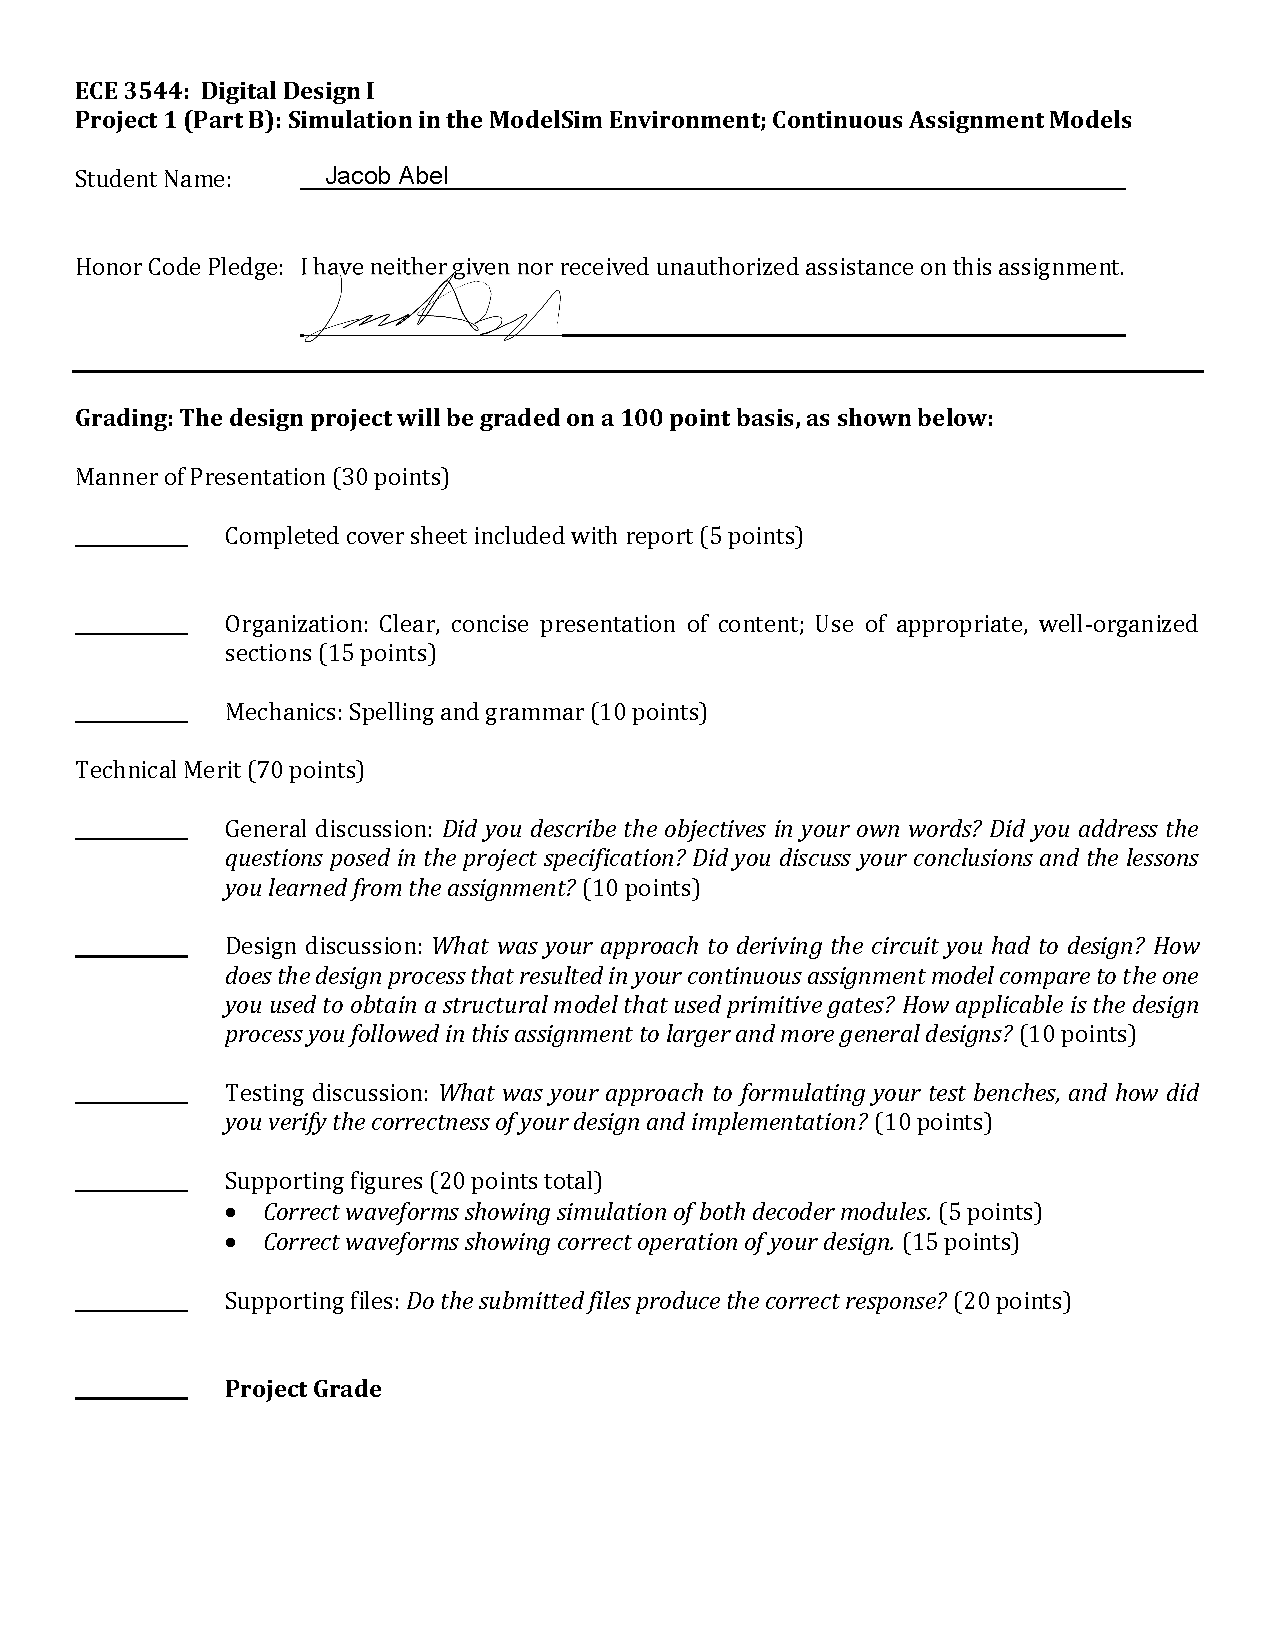
\includepdf[noautoscale]{CoverSheet.pdf}

\maketitle
\begin{raggedright}

\section*{Objective}

The objective of this project is to demonstrate basic competence with the Continuous Assignment Verilog Paradigm. Additionally this project demonstrates the functional equivalence between Continuous Assignment and Structural Verilog Paradigms.

\section{Decoder Simulations}
\begin{center}
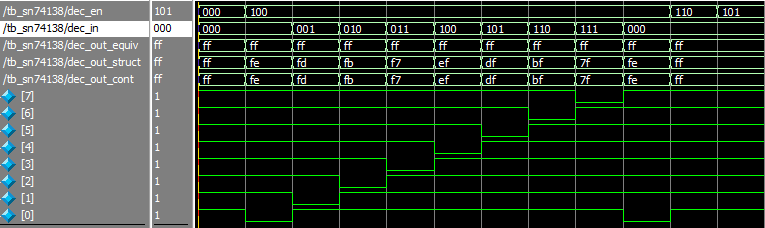
\includegraphics[width=\textwidth]{tb_3to8}
74138 3-to-8 Decoder Test-Bench Waveform
\end{center}

\begin{center}
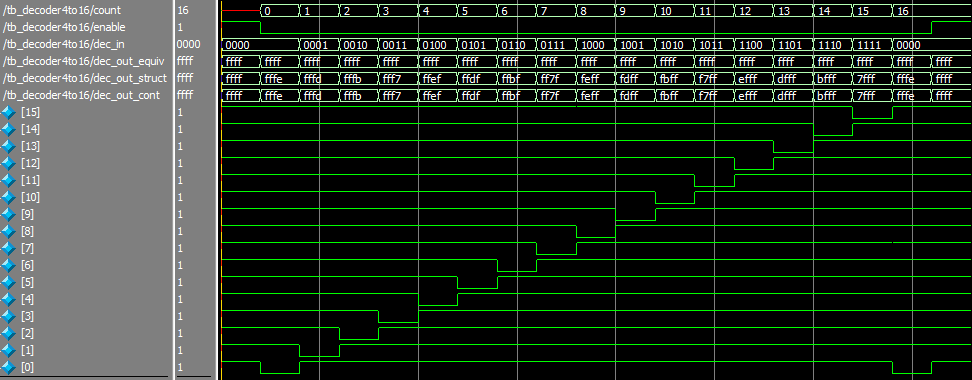
\includegraphics[width=\textwidth, height=\textheight, keepaspectratio=true]{tb_4to16}
4-to-16 Decoder Test-Bench Waveform
\end{center}

The test-benches were adapted to XNOR the outputs of the structural and continuous assignment implementation results. As evidenced by the simulation waveforms, this Continuous Assignment implementation is functionally equivalent to the Structural Verilog implementation of Project 1-A.

\clearpage

\section{Rock Paper Scissors Design}
\textit{The following project description is identical to that of Project 1-A. This implementation of the project must be implemented in Continuous Assignment logic unlike the Structural Verilog of Project 1-A.}


The project requires that a combinatorial circuit be designed that computes the results of a "Rock, Paper, Scissors" game. The circuit accepts two inputs: \texttt{player\_a[1:0]} and \texttt{player\_b[1:0]} and outputs three 1-bit outputs: \texttt{player\_a\_wins}, \texttt{player\_b\_wins}, and \texttt{tie\_game}. The standard rules of the game apply: 
\begin{itemize}
\item Rock beats Scissors
\item Scissors beat Paper
\item Paper beats Rock
\end{itemize}

The values of the input moves are as follows.
\begin{center}
\begin{tabular}{|c|c|c|c|}
\hline 
Move & Rock & Paper & Scissors \\ 
\hline 
Input Value & 11 & 10 & 00 \\ 
\hline 
\end{tabular} 
\end{center}

\subsection*{Design Process Reflection}

The design process for this project was far better adapted to a mid to large scale design project than the process from Project 1-A. This process focused around adapting the test bench to easily demonstrate equivalence to an already proven functional design such as the previously implemented Structural Verilog "Rock, Paper, Scissors" module. Once an equivalence test could be established it became trivial to validate functionality.

The strategy for the design of the actual implementation module was taking the implementation from Project 1-A and condensing it into Continuous Assignment logic. The fundamental structure of the module was roughly the same as in Project 1-A however all the logic was condensed into 5 assign statements. The first two established the hands of the players and the remaining assigns handle the actual game itself. At this point debugging was remarkably easy as any deviation showed up glaringly obvious in the equivalence waveform. Both through conversion from Structural Verilog and in the creation of new modules, Continuous Assignment is significantly more efficient both from a development, readability, and maintainability standpoint.

This design process can work well for large scale designs as it is more or less an adaptation of unit tests from software development. With some additional boilerplate, this design process can easily be extended from simply proving equivalence to serving as a proper unit test suite. Additionally it could be extended to sum all test results and output whether all tests passed.  
\clearpage
\section{Rock Paper Scissors Simulation}
\begin{center}
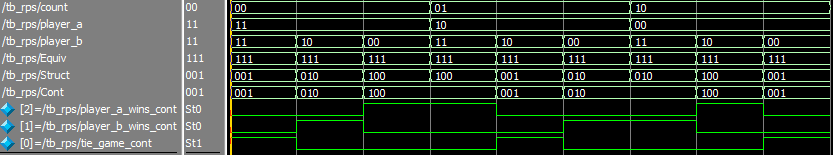
\includegraphics[width=\textwidth]{tb_rps}
Rock Paper Scissors Simulation
\end{center}

The simulation demonstrates that the Continuous Assignment Implementation(\texttt{Cont}) matches the intended behaviour and is equivalent to the Structural Verilog Implementation(\texttt{Struct}). The test bench was designed to cover all possible inputs while minimising repetition. The test bench is the same as the test bench from Project 1-A with an XNOR comparison waveform (\texttt{Equiv}) added to demonstrate equivalence between the Structural Verilog and Continuous Assignment waveforms.

\section{Conclusion}

This project demonstrated that equivalence between varying module implementations can be easily proven. Additionally it demonstrated that structural Verilog can be easily converted to continuous assignment logic and in doing so greatly improves both readability and conciseness. This project overall can be considered a success. Unlike the prior project, sufficient time was allotted for completion and the decreased stress due to a less impending deadline resulted in both less errors and more accurate debugging.


\end{raggedright}
\end{document}
